\chapter{Sujet du stage}
\label{chap:subject}

  \section{Contexte de l'étude}

    Pour répondre à ces enjeux de passage à l'échelle et de consommation
    énergétique, l'équipe ALSOC du LIP6 participe à deux projets européens
    successifs: TSAR~\cite{tsar2008} et SHARP~\cite{sharp2012}. Ces projets,
    pour le LIP6, ont pour but de fournir une architecture de processeur, TSAR,
    de plusieurs centaines de c\oe urs, et un système d'exploitation pour gérer
    efficacement cette nouvelle architecture.

    Notre travail portera sur ALMOS, dont l'architecture va évoluer vers celle
    d'un multi-noyau, et plus particulièrement sur la migration de tâches entre
    différentes instances du noyau. Nous allons dans un premier temps présenter
    l'architecture matérielle TSAR. L'étude de cette dernière est essentielle
    pour bien comprendre les enjeux pour ALMOS. Ensuite nous présenterons le
    noyau ALMOS, et notamment son cycle de vie, et enfin nous concluerons sur le
    travail que nous allons effectuer dans le cadre de ce stage.
  

    \subsection{L'architecture TSAR}
    \label{sec:tsar}

      TSAR est l'architecture d’un processeur multi-c\oe urs cc-NUMA homogène
      pouvant intégrer jusqu’à 1024 c\oe urs~\cite{greiner2009tsar}. Cette
      architecture est le résultat de deux projets de recherche européens
      MEDEA+~\cite{tsar2008,sharp2012} dont les principaux partenaires
      industriels sont BULL, Philips et THALES, et dont les partenaires
      académiques sont le LIP6 et le CEA-Leti. La figure \ref{fig:tsar} est un
      aperçu global de l'architecture TSAR. Il s'agit d'un ensemble de clusters
      interconnectés par un NoC DSPIN. Chaque c\oe ur dispose de ses propres
      caches L1 indexés en adresses physiques (données et instructions
      séparéess) et d'une MMU. La cohérence des caches de premier niveau de tous
      les c\oe urs ainsi que des TLBs est assurée par un protocole matériel
      nommé DHCCP. Une description complète de cette architecture est disponible
      sur le site du projet TSAR~\cite{tsar2008web}.

      \begin{figure}[ht]
        \centering 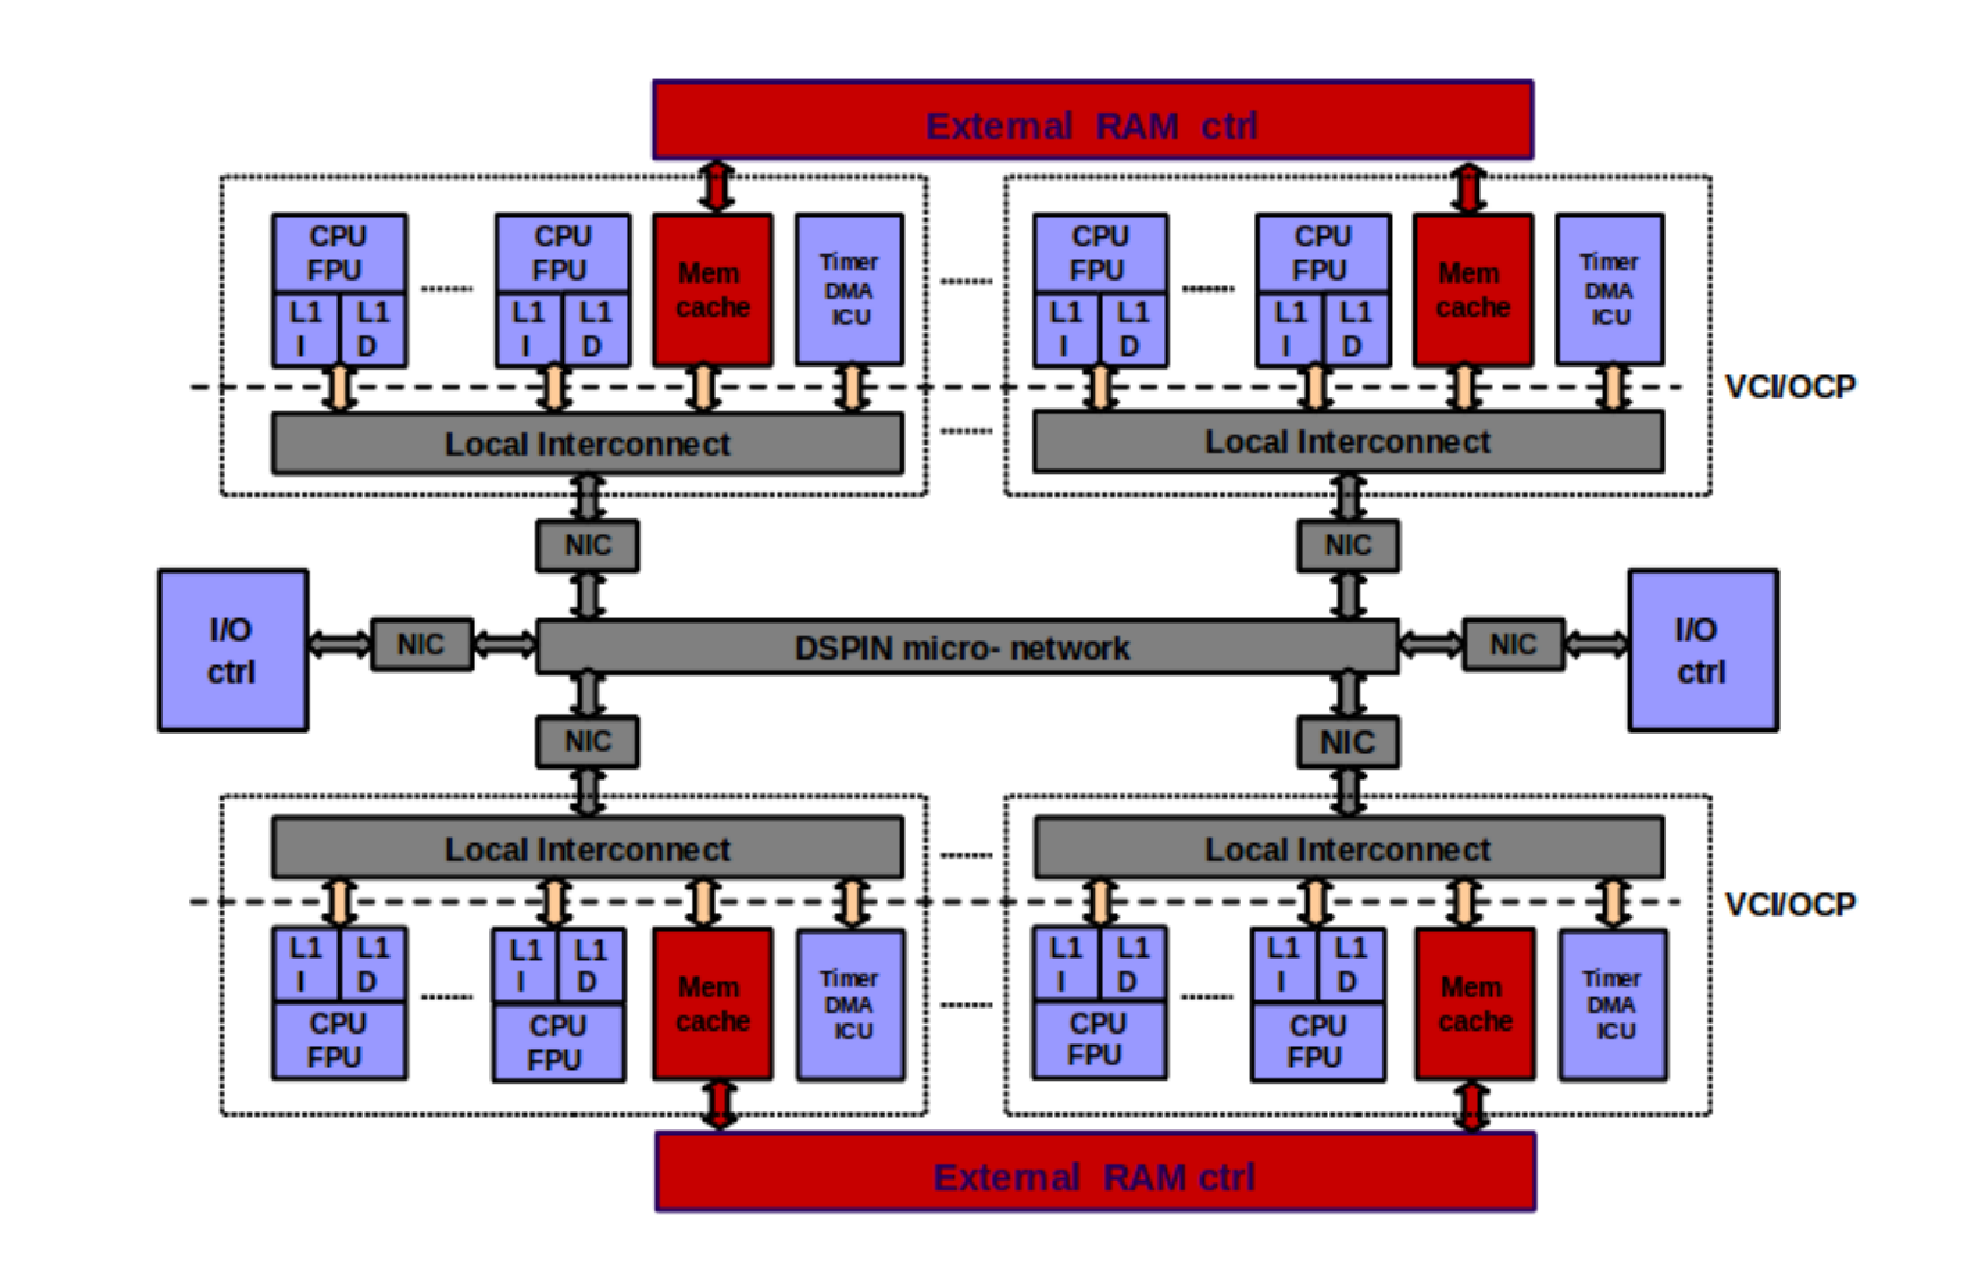
\includegraphics[scale=0.2]{include/img/tsar.png}
        \caption{Schéma global de l'architecture TSAR~\citep{greiner2009tsar}.}
        \label{fig:tsar}
      \end{figure}

      Dans la suite de ce document, on considére la version TSAR-Leti comme
      étant l'architecture de référence. Celle-ci contient jusqu'à 1024 c\oe urs
      MIPS32 répartis en 256 clusters de 4 c\oe urs chacun. La mémoire physique
      adressable est de 1To, et chaque cluster gère un segment de 4Go


    \subsection{Le noyau ALMOS}
    \label{sec:almos}

      Le noyau ALMOS~\cite{almaless2011almos,almaless2014universite} est un
      noyau monolithique expérimental developpé au LIP6 par l'équipe ALSOC
      depuis 2011. Sujet de thèse de Ghassan Almaless, le développement est
      maintenant à la charge de Mohamed Karaoui (système de fichiers) et Clément
      Devigne (exécution de machines virtuelles). Le but d'ALMOS est de répondre
      à la problématique de la localité des accès mémoires dans les machines
      cc-NUMA. Une des particularités dans les choix architecturaux d'ALMOS est
      d'avoir développé un noyau monolithique. Il respecte la norme
      POSIX~\cite{posix2013} et implémente différentes libraires:
      \texttt{libpthread, mpi, openMP}\ldots Le but premier d'ALMOS est de
      garantir un passage à l'échelle et une conservation de la localité des
      accès mémoires. Pour cela, le noyau intègre trois nouveaux mécanismes:
      \benumline \item les clusters managers \item les réplica-noyau \item une
      nouvelle stratégie d'allocation mémoire (\textit{Auto-Next-Touch})
      \eenumline.


    \subsection{Limitations de la version initiale}

      Développé initialement sur une architecture avec 4Go de mémoire physique,
      le noyau ne peut pas supporter plus de 4Go de mémoire vive. L'objectif
      visé n'était pas de supporter le tera-octet de mémoire de TSAR, mais de
      supporter le passage à l'échelle de plusieurs centaines de c\oe
      urs. Ainsi, un des premiers problèmes d'ALMOS est le mapping de l'espace
      virtuel. En effet, lors de la phase de boot, ce dernier cherche à mapper
      toute la mémoire physique du cluster de boot dans son espace
      virtuel. Contraitement aux noyaux ``classiques'', ALMOS s'accorde 2Go
      d'espace virtuel au lieu de 1. Donc, si ce cluster possède (au moins) 2Go
      de mémoire physique, l'ensemble du noyau est mappé dans ce seul
      cluster. Enfin, cela ne laisse que 2Go de mémoire virtuelle pour les
      applications utilisateur.


    \subsection{Contributions de François \citeauthor{guerret2014exploitation}}

      La gestion d'une telle quantité de mémoire fût le sujet de stage de
      François~\citet{guerret2014exploitation} en 2014. Ce dernier proposa
      différents changements pour ALMOS (figure~\ref{fig:almos-guerret}) :
      \benumline \item réduire l'espace virtuel noyau à 1Go \item répartir cet
      espace virtuel entre les clusters \item sortir de l'espace virtuel les
      structures de données du noyau de taille importante \eenumline.

      \begin{paragraph}{Répartition de l'espace d'adressage noyau:}
        Elle est calculée en fonction du nombre de clusters de l'architecture
        ($\frac{\text{Taille virtuelle}}{\text{Nb clusters}}$). Pour une
        architecture TSAR-Leti 40 bits, on dispose de 256 clusters, on a donc
        $\frac{1000}{256}\approx4$Mo d'espace virtuel pour le noyau par cluster.
      \end{paragraph}

      \begin{figure}[ht]
        \centering 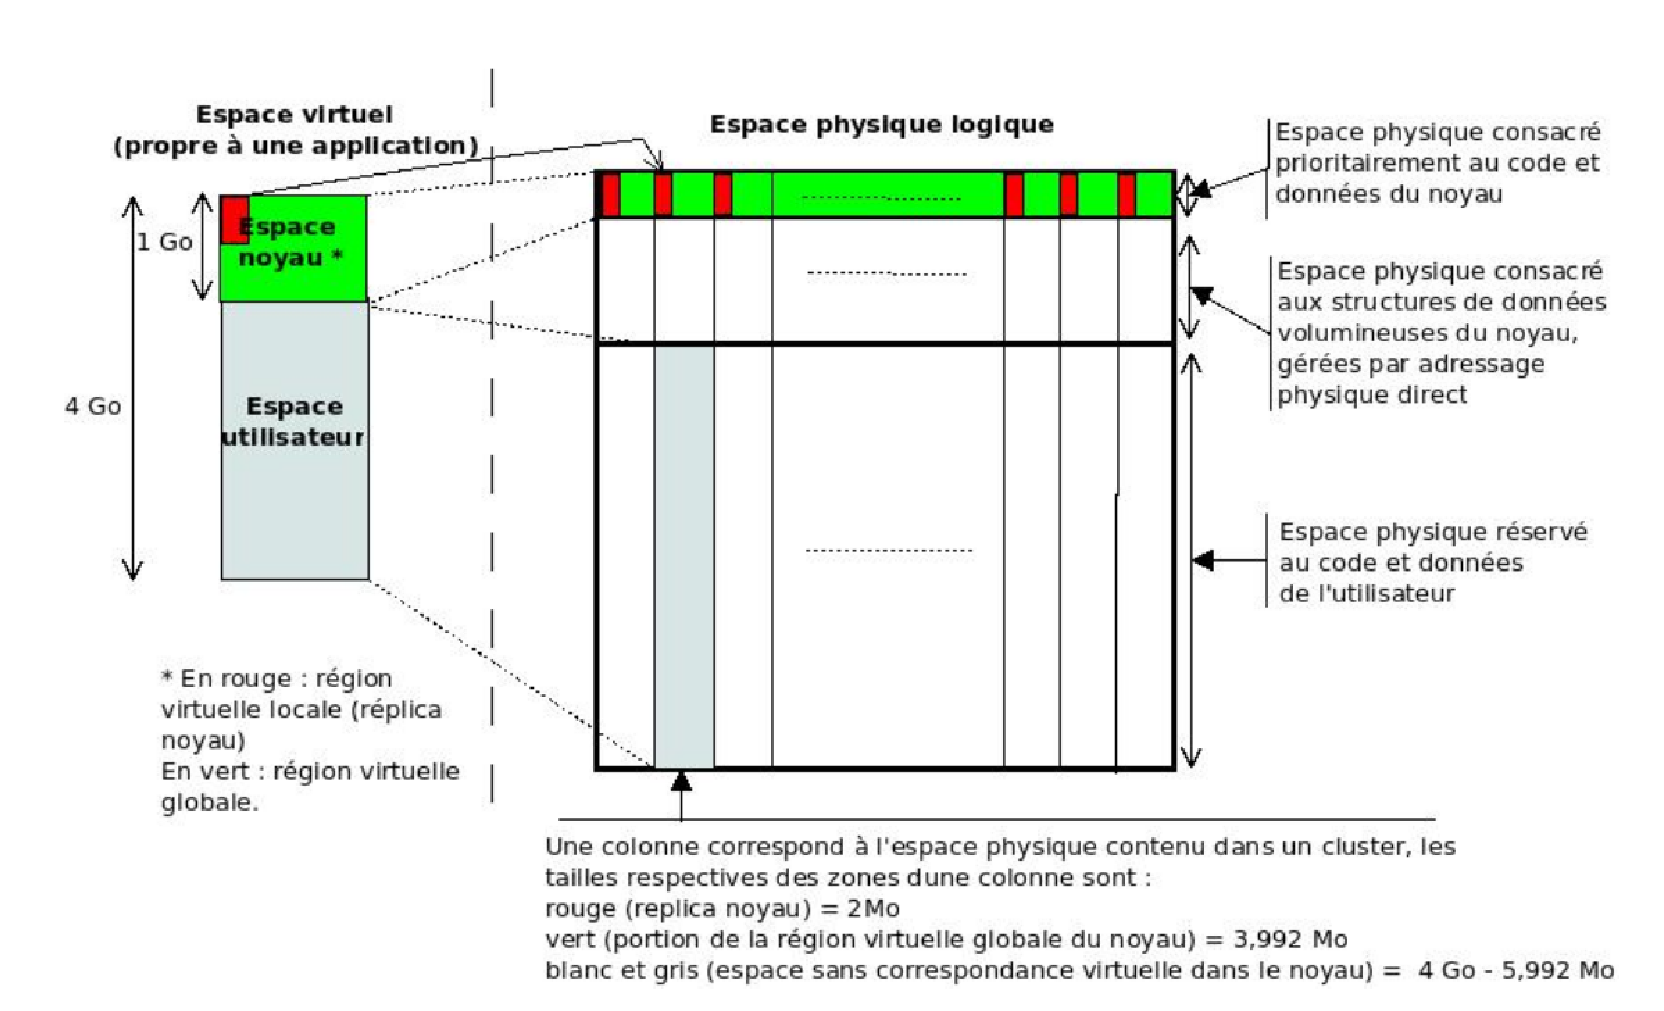
\includegraphics[scale=0.3]{include/img/almos-guerret}
        \caption{Répartition de l'espace virtuel du noyau tel que proposé par
          François \citet{guerret2014exploitation}.}
        \label{fig:almos-guerret}
      \end{figure}

      \begin{paragraph}{Gestion en adressage physiques de structures de données:}
        Avec seulement 4Mo d'espace virtuel pour le noyau par clusters,
        certaines structures de données ne pouvent plus être contenues dans un
        si petit espace, comme par exemple la table des pages d'un
        processus. Celle-ci, une fois pleine\footnote{Ce cas n'arrive jamais,
          mais il est néanmoins théoriquement possible}, peut atteindre une
        taille maximale de 8Mo. De plus, chaque processus dispose de sa propre
        table des pages. Il est techniquement impossible de stocker 8Mo dans
        4Mo, François a donc choisi de sortir cette structure de l'espace
        virtuel.

        La seconde structure de données problématique est la table des
        descripteurs de pages physiques. Les noyaux monolithiques, dont ALMOS,
        ont fait le choix de décrire dans une structure à plat toutes les pages
        physiques qu'offre la mémoire. Ainsi, pour décrire le tera-octet de
        mémoire offert par TSAR, il est nécessaire d'utiliser 14Go de mémoire,
        soit 56Mo par cluster. Une fois de plus, il est impossible de stocker
        cette structure dans l'espace virtuel noyau. Celle-ci en a donc été
        sortie, et est gérée en adressage physique.
      \end{paragraph}

      \begin{paragraph}{Résultats:}
        Ce travail n'a malheureusement pas donné lieu à une solution
        fonctionnelle. La gestion par des adresses physiques de ces deux
        structures s'est avérée être très compliquée et nécessitait de recoder
        une partie conséquente du noyau. Le principal inconvénient de ce choix
        est le parcours de listes: il est nécessaire de vérifier que chaque
        élément n'est pas une structure gérée physiquement avant de pouvoir y
        accéder. Cela allourdi considérablement l'opération, cette solution fût
        donc abandonnée. Néanmoins, elle a posée les bases de la version
        suivante d'ALMOS.
      \end{paragraph}


  \section{Définition et analyse du problème}      

    \subsection{Passage au mode multi-noyau}
    \label{sec:multi-noyau}

      La version actuelle d'ALMOS proposée par Mohamed Karaoui supprime
      totalement l'espace virtuel pour le noyau. Ce dernier fonctionne
      entièrement en adressage physique et de ce fait passe en mode multi-noyau,
      avec une instance de noyau par cluster. Ces changements permettent de
      gérer toute la mémoire physique de la plateforme TSAR, puisque:
      \benumline \item chaque cluster dispose de 4Go de mémoire physique \item
      on a un noyau par cluster \item le noyau peut gérer 4Go de
      mémoire\eenumline. Ces changements permettent également de laisser 4Go de
      mémoire virtuelle\footnote{Modulo une page de petite taille (4Ko) pour
        faire le passage entre le mode utilisateur et le mode noyau} à
      l'utilisateur puisque le noyau ne l'utilise plus.\\

      En revanche, cette solution soulève une difficulté majeure. En choisissant
      de clusteriser le noyau, on rend impossible la communication directe par
      simples load-store à la mémoire des clusters voisins. En effet, avec un
      noyau par cluster, les espaces d'adressage deviennent propres à ces
      derniers, et la vision simple d'un espace d'adressage unique entre les
      clusters n'existe plus. On ne peut donc plus accéder aux éléments des
      autres clusters de manière directe et transparente. Il existe alors deux
      méthodes complémentaires:\benumline \item utiliser une propriété du cache
      L1 de TSAR permettant de former une adresse physique quelconque ou \item
      utiliser le passage de messages entre les instances du noyau\eenumline.\\

      Une seconde conséquence de ce choix est d'avoir rendu non fonctionnelle la
      migration de processus et de threads entre les clusters (la migration
      entre c\oe urs d'un même cluster est toujours fonctionnelle). Dans la
      version initiale d'ALMOS, cette migration se faisait:\benumline \item en
      stoppant le processus sur le c\oe ur concerné puis \item en l'ajoutant
      dans la liste des processus du c\oe ur distant et\item en relancant son
      exécution sur ce nouveau c\oe ur\eenumline. L'ajout du processus dans
      cette liste est possible uniquement parce que le noyau est en mémoire
      virtuelle. Il peut ainsi accéder au \textit{core-manager} du cluster
      destinataire sans se rendre compte que celui-ci est distant, et lui
      ajouter la \texttt{struct task} du processus à migrer. Les pages physiques
      du processus seront ensuite migrées via la stratégie
      \textit{Auto-Next-Touch\footnote{Non détaillée dans ce
          rapport. Voir~\citep{almaless2014universite}.}}.

    \subsection{Contributions}

      En choisissant de passer ALMOS en mode multi-noyau, les clusters sont tous
      gérés par un noyau différent. Ils ont par conséquent des espaces
      d'adressages différents, ce qui invalide les mécanismes de migration de
      processus ou de threads. C'est à cette problématique que nous allons
      répondre.


  \nomenclature{cc-NUMA}{Cache Coherent Non-Uniform Memory Access}
  \nomenclature{NoC}{Network on Chip}
  \nomenclature{DSPIN}{Distributed Scalable Predictable Integrated Network}
  \nomenclature{MMU}{Memory Management Unit}
  \nomenclature{TLB}{Translation Lookaside Buffer}
  \nomenclature{DHCCP}{Distributed Hybrid Cache Coherence Protocol}
  \nomenclature{POSIX}{Portable Operating System Interface}
